\section{Theorie}
\label{sec:theorie}

Im Folgenden sollen sowohl $\gamma$- als auch $\beta$-Strahlung und ihre Eigenschaften 
näher betrachtet werden. \\

Die $\gamma$-Strahlung dient dabei als Beispiel für Photonenstrahlung,
die $\beta$-Strahlung als Beispiel für Teilchenstrahlung.

\subsection*{$\gamma$-Strahlung}

Zunächst soll der Fokus auf die $\gamma$-Strahlung gerichtet werden.

\subsubsection*{Wirkungsquerschnitt und Absorptionsgesetz}

Bei der Wechselwirkung eines Teilchenstrahls mit einer Materieschicht
kommt es zu einer Verringerung der Teilchenzahl pro Zeit und Fläche, 
eine Abnahme der Strahlungsintensität.
Der Wirkungsquerschnitt $\sigma$ stellt dabei ein Maß für die 
Wechselwirkungshäufigkeit dar. \\

Die Wahrscheinlichkeit, dass ein einfallendes Teilchen auf
die fikitve Fläche $\sigma$ des Querschnitts $F$ und der Dicke $D$
eine Wechselwirkung aulöst, wenn die Fläche $n$ Materieteilchen pro
Volumen enthält, ist durch

\begin{equation}
    W = \frac{n F D \sigma}{F} = n D \sigma
\end{equation}
gegeben.
Eine schematische Darstellung dieser Flächen $\sigma$ sei in
\autoref{fig:abb1} dargestellt.

\begin{figure}
    \centering
    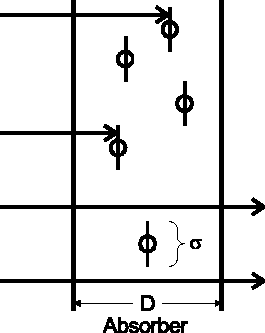
\includegraphics{figures/abb1.pdf}
    \caption{Schematische Darstellung einer Absorberschicht der Dicke $D$\cite{ap04}.}
    \label{fig:abb1}
\end{figure}

Pro Zeiteinheit finden dann, bei $N_0$ eintreffenden Teilchen,
\begin{equation}
    N = N_0 n D \sigma
    \label{eq:wechselwirkgamma}
\end{equation}
Wechselwirkungen statt. \\

Bei einem realen Absorber muss die Summation aller Schichten $\sigma$
über infinitesimale Schichten $\dif x$ stattfinden.
Nach der Integration über alle Schichten folgt daraus

\begin{equation}
    N(D) = N_0 \mathrm{e}^{-n \sigma D} \,.
    \label{eq:wechselwirkgammaexp}
\end{equation} \\

Dabei ist der Absorptionskoeffizient $\mu$ 
bei der Schichtdicke $D_{1/2}$ definiert als
\begin{equation*}
    \mu := n \sigma = D_{1/2} \ln 2 \,.
\end{equation*} \\

Zur Bestimmung der Teilchenzahl im Absorber der Ordnungszahl $\text{z}$ und
dem Molvolumen $V_{\text{Mol}}$ bzw. der Dichte $\rho$ und dem
Molekulargewicht $M$ dient
\begin{equation*}
    n = \frac{\text{z} N_L}{V_{\text{Mol}}} = \frac{\text{z} N_L \rho}{M} \,,
\end{equation*}
wobei $N_L$ die Loschmidtsche Zahl darstellt. \\

Der Wirkungsquerschnitt ergibt sich damit zu
\begin{equation}
    \sigma = \frac{\mu}{n} = \frac{\mu N}{z N_L \rho} \,.
    \label{eq:wirkungsquerschnitt}
\end{equation}

Jedoch stellt \eqref{eq:wirkungsquerschnitt} nur eine grobe Näherung,
keine exakte Berechnung des Wirkungsquerschnitts dar. \\


\subsubsection*{Eigenschaften der $\gamma$-Strahlung}

Geht ein Atom in einen energetisch günsigeren Zustand über, wird die
überschüssige Energie in Form von $\gamma$-Quanten abgegeben.
Diese $\gamma$-Quanten besitzen sowohl Teilchen- als auch Wellencharakter,
ihre Energie bei der Lichtgeschwindigkeit $\mathrm{c}$ ist dabei durch
\begin{equation*}
    E_\gamma = \mathrm{h} \nu = \frac{\text{h} \mathrm{c}}{\lambda}
\end{equation*}
gegeben, wobei $\nu$ die Frequenz, $\lambda$ die Wellenlänge 
und $\mathrm{h}$ das Plancksche Wirkungquantum darstellen.
Aufgrund der diskreten Kernenergieniveaus stellt das $\gamma$-Spektrum
eines Kerns ein Linienspektrum scharfer Linien dar.


\subsubsection*{Wechselwirkung mit Materie}

Dringt ein Quant in eine Materieschicht ein, kann es mit den
Elektronen, den Kernen sowie ihren elekrischen Feldern interagieren.
Die dabei möglichen Annihilationsprozesse sowie der inelastischen
und elastischen Streuung sind dabei in \autoref{fig:abb2} dargestellt.

\begin{figure}
    \centering
    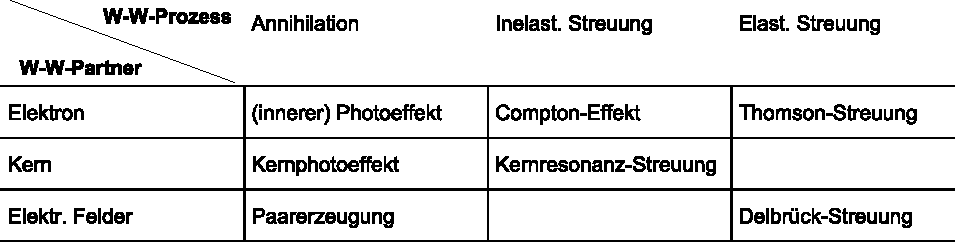
\includegraphics{figures/abb2.pdf}
    \caption{Tabellarische Darstellung der verschiedenen Wechselwirkungsmöglichkeiten von $\gamma$-Strahlung mit Materie\cite{ap04}.}
    \label{fig:abb2}
\end{figure}

Am wichtigsten sind dabei der Photoeffekt, der Comptoneffekt sowie
die Paarbildung.

Beim Photoeffekt wechselwirkt das Photon mit einem Hüllenelektron und
wird dabei vernichtet; das Elektron wird aus seiner Bindung entfernt.
Die Elektronenenerie nach dem Stoß ist dann gegeben durch
\begin{equation*}
    E_{\mathrm{e}} = \mathrm{h} \nu - E_{\mathrm{B}} \,.
\end{equation*} \\

\begin{figure}[H]
    \centering
    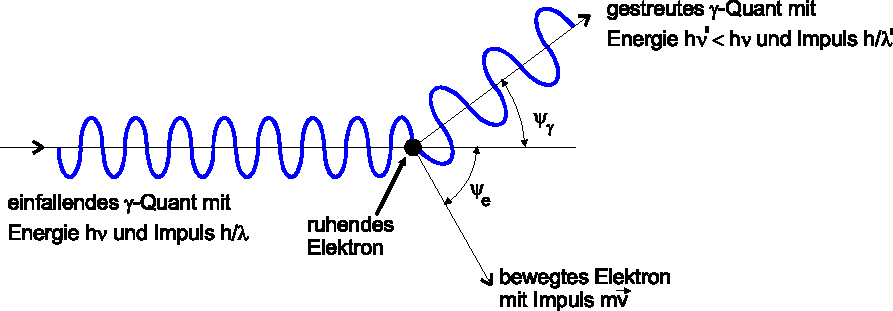
\includegraphics{figures/abb3.pdf}
    \caption{Schematische Darstellung des Comptoneffekts\cite{ap04}.}
    \label{fig:abb3}
\end{figure}

Bei der Streuung eines Quants an einem freien Elektron wird vom
Comptoneffekt gesprochen.


\autoref{fig:abb3} entsprechend gibt das Photon einen Großteil
seiner Energie an das Elektron ab, im Gegensatz zum Photoeffekt
wird das Photon aber nicht vernichtet. \\

Der Wirkungsquerschnitt $\sigma_{\mathrm{com}}$ ist dabei gegeben durch
\begin{equation}
    \sigma_{\mathrm{com}} = 2 \pi r^2_\mathrm{e} 
    \left(\frac{1 + \varepsilon}{\varepsilon^2} 
    \left[\frac{2(1 + \varepsilon)}{1 + 2 \varepsilon} -\frac{1}{\varepsilon}\right]
    + \frac{1}{2 \varepsilon} \ln(1 + 2 \varepsilon) 
    - \frac{1 + 3 \varepsilon}{(1 + 2 \varepsilon)^2}\right)
    \label{eq:wirkungsquercompton}
\end{equation}